

\tikzset{every picture/.style={line width=0.75pt}} %set default line width to 0.75pt        

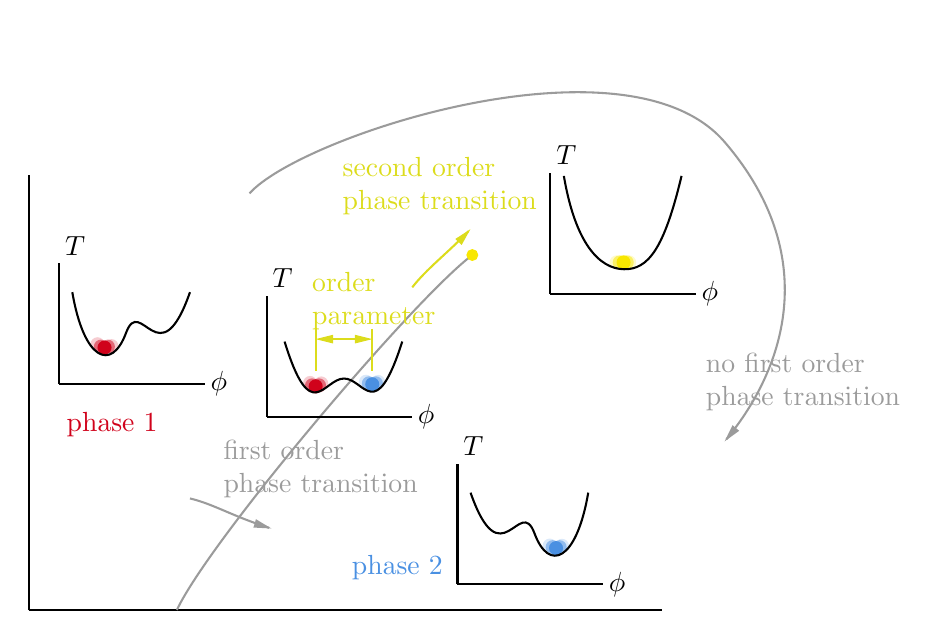
\begin{tikzpicture}[x=0.75pt,y=0.75pt,yscale=-0.7,xscale=0.7]
%uncomment if require: \path (0,399); %set diagram left start at 0, and has height of 399

%Shape: Ellipse [id:dp8966056933022035] 
\draw  [draw opacity=0][fill={rgb, 255:red, 248; green, 231; blue, 0 }  ,fill opacity=1 ] (485.28,134.5) .. controls (485.28,131.83) and (483.11,129.67) .. (480.44,129.67) .. controls (477.78,129.67) and (475.61,131.83) .. (475.61,134.5) .. controls (475.61,137.17) and (477.78,139.33) .. (480.44,139.33) .. controls (483.11,139.33) and (485.28,137.17) .. (485.28,134.5) -- cycle ;
%Shape: Ellipse [id:dp7109493034256176] 
\draw  [draw opacity=0][fill={rgb, 255:red, 248; green, 231; blue, 0 }  ,fill opacity=0.2 ] (489.11,134.5) .. controls (489.11,131.83) and (486.95,129.67) .. (484.28,129.67) .. controls (481.61,129.67) and (479.44,131.83) .. (479.44,134.5) .. controls (479.44,137.17) and (481.61,139.33) .. (484.28,139.33) .. controls (486.95,139.33) and (489.11,137.17) .. (489.11,134.5) -- cycle ;
%Shape: Ellipse [id:dp6253244151348323] 
\draw  [draw opacity=0][fill={rgb, 255:red, 248; green, 231; blue, 0 }  ,fill opacity=0.5 ] (487.44,134.5) .. controls (487.44,131.83) and (485.28,129.67) .. (482.61,129.67) .. controls (479.94,129.67) and (477.78,131.83) .. (477.78,134.5) .. controls (477.78,137.17) and (479.94,139.33) .. (482.61,139.33) .. controls (485.28,139.33) and (487.44,137.17) .. (487.44,134.5) -- cycle ;
%Shape: Ellipse [id:dp8602845534054557] 
\draw  [draw opacity=0][fill={rgb, 255:red, 248; green, 231; blue, 0 }  ,fill opacity=0.2 ] (480.44,134.5) .. controls (480.44,131.83) and (478.28,129.67) .. (475.61,129.67) .. controls (472.94,129.67) and (470.78,131.83) .. (470.78,134.5) .. controls (470.78,137.17) and (472.94,139.33) .. (475.61,139.33) .. controls (478.28,139.33) and (480.44,137.17) .. (480.44,134.5) -- cycle ;
%Shape: Ellipse [id:dp7131013462396065] 
\draw  [draw opacity=0][fill={rgb, 255:red, 248; green, 231; blue, 0 }  ,fill opacity=0.5 ] (482.61,134.5) .. controls (482.61,131.83) and (480.45,129.67) .. (477.78,129.67) .. controls (475.11,129.67) and (472.94,131.83) .. (472.94,134.5) .. controls (472.94,137.17) and (475.11,139.33) .. (477.78,139.33) .. controls (480.45,139.33) and (482.61,137.17) .. (482.61,134.5) -- cycle ;
%Shape: Circle [id:dp547058566666722] 
\draw  [draw opacity=0][fill={rgb, 255:red, 74; green, 144; blue, 226 }  ,fill opacity=1 ] (438.78,331.17) .. controls (438.78,328.5) and (436.61,326.33) .. (433.94,326.33) .. controls (431.28,326.33) and (429.11,328.5) .. (429.11,331.17) .. controls (429.11,333.84) and (431.28,336) .. (433.94,336) .. controls (436.61,336) and (438.78,333.84) .. (438.78,331.17) -- cycle ;
%Shape: Ellipse [id:dp3101275508990131] 
\draw  [draw opacity=0][fill={rgb, 255:red, 74; green, 144; blue, 226 }  ,fill opacity=0.5 ] (436.44,330.5) .. controls (436.44,327.83) and (434.28,325.67) .. (431.61,325.67) .. controls (428.94,325.67) and (426.78,327.83) .. (426.78,330.5) .. controls (426.78,333.17) and (428.94,335.33) .. (431.61,335.33) .. controls (434.28,335.33) and (436.44,333.17) .. (436.44,330.5) -- cycle ;
%Shape: Circle [id:dp7020282078610482] 
\draw  [draw opacity=0][fill={rgb, 255:red, 74; green, 144; blue, 226 }  ,fill opacity=0.5 ] (441.28,330.5) .. controls (441.28,327.83) and (439.11,325.67) .. (436.44,325.67) .. controls (433.78,325.67) and (431.61,327.83) .. (431.61,330.5) .. controls (431.61,333.17) and (433.78,335.33) .. (436.44,335.33) .. controls (439.11,335.33) and (441.28,333.17) .. (441.28,330.5) -- cycle ;
%Shape: Ellipse [id:dp4373949259279002] 
\draw  [draw opacity=0][fill={rgb, 255:red, 74; green, 144; blue, 226 }  ,fill opacity=0.2 ] (442.86,329.58) .. controls (442.86,326.91) and (440.7,324.75) .. (438.03,324.75) .. controls (435.36,324.75) and (433.19,326.91) .. (433.19,329.58) .. controls (433.19,332.25) and (435.36,334.42) .. (438.03,334.42) .. controls (440.7,334.42) and (442.86,332.25) .. (442.86,329.58) -- cycle ;
%Shape: Ellipse [id:dp8592445886281008] 
\draw  [draw opacity=0][fill={rgb, 255:red, 74; green, 144; blue, 226 }  ,fill opacity=0.2 ] (434.44,329.42) .. controls (434.44,326.75) and (432.28,324.58) .. (429.61,324.58) .. controls (426.94,324.58) and (424.78,326.75) .. (424.78,329.42) .. controls (424.78,332.09) and (426.94,334.25) .. (429.61,334.25) .. controls (432.28,334.25) and (434.44,332.09) .. (434.44,329.42) -- cycle ;
%Shape: Circle [id:dp9930826195596292] 
\draw  [draw opacity=0][fill={rgb, 255:red, 208; green, 2; blue, 27 }  ,fill opacity=1 ] (118.33,193.17) .. controls (118.33,190.5) and (120.5,188.33) .. (123.17,188.33) .. controls (125.84,188.33) and (128,190.5) .. (128,193.17) .. controls (128,195.84) and (125.84,198) .. (123.17,198) .. controls (120.5,198) and (118.33,195.84) .. (118.33,193.17) -- cycle ;
%Shape: Circle [id:dp22542225507833424] 
\draw  [draw opacity=0][fill={rgb, 255:red, 208; green, 2; blue, 27 }  ,fill opacity=0.5 ] (120.67,192.5) .. controls (120.67,189.83) and (122.83,187.67) .. (125.5,187.67) .. controls (128.17,187.67) and (130.33,189.83) .. (130.33,192.5) .. controls (130.33,195.17) and (128.17,197.33) .. (125.5,197.33) .. controls (122.83,197.33) and (120.67,195.17) .. (120.67,192.5) -- cycle ;
%Shape: Circle [id:dp9501769788062395] 
\draw  [draw opacity=0][fill={rgb, 255:red, 208; green, 2; blue, 27 }  ,fill opacity=0.5 ] (115.83,192.5) .. controls (115.83,189.83) and (118,187.67) .. (120.67,187.67) .. controls (123.34,187.67) and (125.5,189.83) .. (125.5,192.5) .. controls (125.5,195.17) and (123.34,197.33) .. (120.67,197.33) .. controls (118,197.33) and (115.83,195.17) .. (115.83,192.5) -- cycle ;
%Shape: Circle [id:dp3322722462547172] 
\draw  [draw opacity=0][fill={rgb, 255:red, 208; green, 2; blue, 27 }  ,fill opacity=0.2 ] (113.5,190.83) .. controls (113.5,188.16) and (115.66,186) .. (118.33,186) .. controls (121,186) and (123.17,188.16) .. (123.17,190.83) .. controls (123.17,193.5) and (121,195.67) .. (118.33,195.67) .. controls (115.66,195.67) and (113.5,193.5) .. (113.5,190.83) -- cycle ;
%Shape: Circle [id:dp25465582637170003] 
\draw  [draw opacity=0][fill={rgb, 255:red, 208; green, 2; blue, 27 }  ,fill opacity=0.2 ] (123.17,192.17) .. controls (123.17,189.5) and (125.33,187.33) .. (128,187.33) .. controls (130.67,187.33) and (132.83,189.5) .. (132.83,192.17) .. controls (132.83,194.84) and (130.67,197) .. (128,197) .. controls (125.33,197) and (123.17,194.84) .. (123.17,192.17) -- cycle ;
%Shape: Circle [id:dp8614398233093736] 
\draw  [draw opacity=0][fill={rgb, 255:red, 74; green, 144; blue, 226 }  ,fill opacity=1 ] (312.28,218.42) .. controls (312.28,215.75) and (310.11,213.58) .. (307.44,213.58) .. controls (304.78,213.58) and (302.61,215.75) .. (302.61,218.42) .. controls (302.61,221.09) and (304.78,223.25) .. (307.44,223.25) .. controls (310.11,223.25) and (312.28,221.09) .. (312.28,218.42) -- cycle ;
%Shape: Ellipse [id:dp16657356514972] 
\draw  [draw opacity=0][fill={rgb, 255:red, 74; green, 144; blue, 226 }  ,fill opacity=0.5 ] (309.94,217.75) .. controls (309.94,215.08) and (307.78,212.92) .. (305.11,212.92) .. controls (302.44,212.92) and (300.28,215.08) .. (300.28,217.75) .. controls (300.28,220.42) and (302.44,222.58) .. (305.11,222.58) .. controls (307.78,222.58) and (309.94,220.42) .. (309.94,217.75) -- cycle ;
%Shape: Circle [id:dp5570619668435961] 
\draw  [draw opacity=0][fill={rgb, 255:red, 74; green, 144; blue, 226 }  ,fill opacity=0.5 ] (314.78,217.75) .. controls (314.78,215.08) and (312.61,212.92) .. (309.94,212.92) .. controls (307.28,212.92) and (305.11,215.08) .. (305.11,217.75) .. controls (305.11,220.42) and (307.28,222.58) .. (309.94,222.58) .. controls (312.61,222.58) and (314.78,220.42) .. (314.78,217.75) -- cycle ;
%Shape: Ellipse [id:dp4022683812151078] 
\draw  [draw opacity=0][fill={rgb, 255:red, 74; green, 144; blue, 226 }  ,fill opacity=0.2 ] (316.36,216.83) .. controls (316.36,214.16) and (314.2,212) .. (311.53,212) .. controls (308.86,212) and (306.69,214.16) .. (306.69,216.83) .. controls (306.69,219.5) and (308.86,221.67) .. (311.53,221.67) .. controls (314.2,221.67) and (316.36,219.5) .. (316.36,216.83) -- cycle ;
%Shape: Ellipse [id:dp7153724875575014] 
\draw  [draw opacity=0][fill={rgb, 255:red, 74; green, 144; blue, 226 }  ,fill opacity=0.2 ] (307.94,216.67) .. controls (307.94,214) and (305.78,211.83) .. (303.11,211.83) .. controls (300.44,211.83) and (298.28,214) .. (298.28,216.67) .. controls (298.28,219.34) and (300.44,221.5) .. (303.11,221.5) .. controls (305.78,221.5) and (307.94,219.34) .. (307.94,216.67) -- cycle ;
%Shape: Circle [id:dp8741228306404174] 
\draw  [draw opacity=0][fill={rgb, 255:red, 208; green, 2; blue, 27 }  ,fill opacity=1 ] (263.67,219.83) .. controls (263.67,217.16) and (265.83,215) .. (268.5,215) .. controls (271.17,215) and (273.33,217.16) .. (273.33,219.83) .. controls (273.33,222.5) and (271.17,224.67) .. (268.5,224.67) .. controls (265.83,224.67) and (263.67,222.5) .. (263.67,219.83) -- cycle ;
%Shape: Circle [id:dp3086505521560021] 
\draw  [draw opacity=0][fill={rgb, 255:red, 208; green, 2; blue, 27 }  ,fill opacity=0.5 ] (266,219.17) .. controls (266,216.5) and (268.16,214.33) .. (270.83,214.33) .. controls (273.5,214.33) and (275.67,216.5) .. (275.67,219.17) .. controls (275.67,221.84) and (273.5,224) .. (270.83,224) .. controls (268.16,224) and (266,221.84) .. (266,219.17) -- cycle ;
%Shape: Circle [id:dp9301649922749247] 
\draw  [draw opacity=0][fill={rgb, 255:red, 208; green, 2; blue, 27 }  ,fill opacity=0.5 ] (261.17,219.17) .. controls (261.17,216.5) and (263.33,214.33) .. (266,214.33) .. controls (268.67,214.33) and (270.83,216.5) .. (270.83,219.17) .. controls (270.83,221.84) and (268.67,224) .. (266,224) .. controls (263.33,224) and (261.17,221.84) .. (261.17,219.17) -- cycle ;
%Shape: Circle [id:dp7360361951586791] 
\draw  [draw opacity=0][fill={rgb, 255:red, 208; green, 2; blue, 27 }  ,fill opacity=0.2 ] (259.83,217.5) .. controls (259.83,214.83) and (262,212.67) .. (264.67,212.67) .. controls (267.34,212.67) and (269.5,214.83) .. (269.5,217.5) .. controls (269.5,220.17) and (267.34,222.33) .. (264.67,222.33) .. controls (262,222.33) and (259.83,220.17) .. (259.83,217.5) -- cycle ;
%Shape: Circle [id:dp8173345938838197] 
\draw  [draw opacity=0][fill={rgb, 255:red, 208; green, 2; blue, 27 }  ,fill opacity=0.2 ] (267.5,217.83) .. controls (267.5,215.16) and (269.66,213) .. (272.33,213) .. controls (275,213) and (277.17,215.16) .. (277.17,217.83) .. controls (277.17,220.5) and (275,222.67) .. (272.33,222.67) .. controls (269.66,222.67) and (267.5,220.5) .. (267.5,217.83) -- cycle ;
%Straight Lines [id:da7634021733400376] 
\draw    (71,374) -- (507,374) ;
%Straight Lines [id:da917578897566115] 
\draw    (71,374) -- (71,74.44) ;
%Curve Lines [id:da196714613363133] 
\draw [color={rgb, 255:red, 155; green, 155; blue, 155 }  ,draw opacity=1 ]   (173,373.67) .. controls (196,325) and (336.33,159.44) .. (376.33,129.44) ;
%Straight Lines [id:da6510956947903301] 
\draw    (92,218) -- (192,218) ;
%Straight Lines [id:da09970468999575277] 
\draw    (92,218) -- (92,135) ;
%Curve Lines [id:da16068322492876574] 
\draw    (101,155) .. controls (109,202) and (128,210) .. (138,183) .. controls (148,156) and (161,215) .. (182,155) ;
%Straight Lines [id:da20123834302706678] 
\draw [color={rgb, 255:red, 248; green, 231; blue, 0 }  ,draw opacity=1 ]   (376.33,129.44) ;
\draw [shift={(376.33,129.44)}, rotate = 0] [color={rgb, 255:red, 248; green, 231; blue, 0 }  ,draw opacity=1 ][fill={rgb, 255:red, 248; green, 231; blue, 0 }  ,fill opacity=1 ][line width=0.75]      (0, 0) circle [x radius= 3.35, y radius= 3.35]   ;
%Straight Lines [id:da025415533142057578] 
\draw    (366.11,356) -- (466.11,356) ;
%Straight Lines [id:da8958644995764178] 
\draw    (366.11,356) -- (366.11,273) ;
%Curve Lines [id:da7155920662475712] 
\draw    (456.11,293) .. controls (448.11,340) and (429.11,348) .. (419.11,321) .. controls (409.11,294) and (396.11,353) .. (375.11,293) ;
%Straight Lines [id:da26282833471750533] 
\draw    (234.78,240.67) -- (334.78,240.67) ;
%Straight Lines [id:da14094577118170237] 
\draw    (234.78,240.67) -- (234.78,157.67) ;
%Curve Lines [id:da196413795037508] 
\draw    (328.11,189) .. controls (309.58,246.92) and (302,214.44) .. (288,214.44) .. controls (274,214.44) and (265.33,248.17) .. (247.11,189) ;
%Straight Lines [id:da09064080101133798] 
\draw    (430,156) -- (530,156) ;
%Straight Lines [id:da10568918530924343] 
\draw    (430,156) -- (430,73) ;
%Curve Lines [id:da06934572662234562] 
\draw    (439.33,75) .. controls (447.33,122) and (464,138.89) .. (480.67,139.22) .. controls (497.33,139.56) and (508.33,125.22) .. (520.33,75) ;
%Straight Lines [id:da06092546267448662] 
\draw [color={rgb, 255:red, 220; green, 220; blue, 28 }  ,draw opacity=1 ]   (268.5,180.33) -- (268.5,209) ;
%Straight Lines [id:da26006180280306035] 
\draw [color={rgb, 255:red, 220; green, 220; blue, 28 }  ,draw opacity=1 ]   (307.5,180.33) -- (307.5,209) ;
%Straight Lines [id:da8400902867725275] 
\draw [color={rgb, 255:red, 220; green, 220; blue, 28 }  ,draw opacity=1 ]   (270.5,187.33) -- (305.5,187.33) ;
\draw [shift={(307.5,187.33)}, rotate = 180] [fill={rgb, 255:red, 220; green, 220; blue, 28 }  ,fill opacity=1 ][line width=0.08]  [draw opacity=0] (12,-3) -- (0,0) -- (12,3) -- cycle    ;
\draw [shift={(268.5,187.33)}, rotate = 0] [fill={rgb, 255:red, 220; green, 220; blue, 28 }  ,fill opacity=1 ][line width=0.08]  [draw opacity=0] (12,-3) -- (0,0) -- (12,3) -- cycle    ;
%Curve Lines [id:da22098652196230462] 
\draw [color={rgb, 255:red, 220; green, 220; blue, 28 }  ,draw opacity=1 ]   (335,151.67) .. controls (344.7,139.06) and (360.05,127.39) .. (373.73,113.01) ;
\draw [shift={(375,111.67)}, rotate = 133.03] [fill={rgb, 255:red, 220; green, 220; blue, 28 }  ,fill opacity=1 ][line width=0.08]  [draw opacity=0] (12,-3) -- (0,0) -- (12,3) -- cycle    ;
%Curve Lines [id:da3579393008155043] 
\draw [color={rgb, 255:red, 155; green, 155; blue, 155 }  ,draw opacity=1 ]   (182,297) .. controls (197.68,300.59) and (211.44,309.31) .. (236.45,317.19) ;
\draw [shift={(238,317.67)}, rotate = 197.1] [fill={rgb, 255:red, 155; green, 155; blue, 155 }  ,fill opacity=1 ][line width=0.08]  [draw opacity=0] (12,-3) -- (0,0) -- (12,3) -- cycle    ;
%Curve Lines [id:da6338099051331245] 
\draw [color={rgb, 255:red, 155; green, 155; blue, 155 }  ,draw opacity=1 ]   (223,87) .. controls (258,47.67) and (483,-26.33) .. (550,51.67) .. controls (616.33,128.89) and (592.49,206.11) .. (551.25,256.16) ;
\draw [shift={(550,257.67)}, rotate = 310.03] [fill={rgb, 255:red, 155; green, 155; blue, 155 }  ,fill opacity=1 ][line width=0.08]  [draw opacity=0] (12,-3) -- (0,0) -- (12,3) -- cycle    ;

% Text Node
\draw (95,235.67) node [anchor=north west][inner sep=0.75pt]  [color={rgb, 255:red, 208; green, 2; blue, 27 }  ,opacity=1 ] [align=left] {phase 1};
% Text Node
\draw (291.33,334) node [anchor=north west][inner sep=0.75pt]  [color={rgb, 255:red, 74; green, 144; blue, 226 }  ,opacity=1 ] [align=left] {phase 2};
% Text Node
\draw (236.78,154.27) node [anchor=south west] [inner sep=0.75pt]    {$T$};
% Text Node
\draw (336.78,240.67) node [anchor=west] [inner sep=0.75pt]    {$\phi $};
% Text Node
\draw (203,255) node [anchor=north west][inner sep=0.75pt]  [color={rgb, 255:red, 155; green, 155; blue, 155 }  ,opacity=1 ] [align=left] {first order \\phase transition};
% Text Node
\draw (94,131.6) node [anchor=south west] [inner sep=0.75pt]    {$T$};
% Text Node
\draw (194,218) node [anchor=west] [inner sep=0.75pt]    {$\phi $};
% Text Node
\draw (368.11,269.6) node [anchor=south west] [inner sep=0.75pt]    {$T$};
% Text Node
\draw (468.11,356) node [anchor=west] [inner sep=0.75pt]    {$\phi $};
% Text Node
\draw (432,69.6) node [anchor=south west] [inner sep=0.75pt]    {$T$};
% Text Node
\draw (532,156) node [anchor=west] [inner sep=0.75pt]    {$\phi $};
% Text Node
\draw (285,60) node [anchor=north west][inner sep=0.75pt]  [color={rgb, 255:red, 220; green, 220; blue, 28 }  ,opacity=1 ] [align=left] {second order \\phase transition};
% Text Node
\draw (264,139) node [anchor=north west][inner sep=0.75pt]  [color={rgb, 255:red, 220; green, 220; blue, 28 }  ,opacity=1 ] [align=left] {order \\parameter};
% Text Node
\draw (535,195) node [anchor=north west][inner sep=0.75pt]  [color={rgb, 255:red, 155; green, 155; blue, 155 }  ,opacity=1 ] [align=left] {no first order \\phase transition};


\end{tikzpicture}
